\chapter{JPEG Artifact Removal}
\section{Introduction}
Despite the existence of better compression algorithms, use of the JPEG compression algorithm is ubiquitous: it is the most commonly used image compression algorithm.  Overzealous JPEG compression can produce visible distortions, and image restoration from these distortions is a challenging problem. There are two aspects of JPEG compression which make the restoration process more challenging than simpler restoration problems like deblurring or removing salt-and-pepper noise: JPEG's block-based approach is not spatially invariant, and the quantization is nonlinear. This chapter describes a novel approach to address the challenges of JPEG image restoration using the ADMM-based convolutional sparse coding for a multi-layer dictionary model.
\section{JPEG Algorithm}

The JPEG compression process begins with an RGB image input, and consists of five steps. The first is a color transformation, transitioning from RGB to YUV. Then, the U and V color channels are downsampled.  The DCT for each $8 \times 8$ block is computed (separately for each channel).  The DCT coefficients are then quantized using a quantization matrix determined by a user-chosen JPEG quality factor. Finally, these quantized coefficients are reordered and encoded using a lossless variable length coding process.

The standard reconstruction process reverses the lossless encoding, computes the IDCT of the blocks, upsamples the color channels, and reverses the color transform.
\section{Modeling Compressed JPEG Images}
Some researchers have observed that convolutional dictionary models struggle with large smooth components of signals \cite{garcia2018convolutional}, likely due to the fact that shifted versions of smooth filters have high coherence.

For this reason, it is often a good idea to subtract a smoothed version $\vs_{\text{smth}}$ of the signal, and only apply the dictionary model to the residual $\vs_{\text{rough}}$.
%
\begin{equation}
\vs_{\text{clean}} = \vs_{\text{smth}} + \vs_{\text{rough}}
\end{equation}
%
\begin{equation}
\vs_{\text{rough}} \approx \mD_1\vx_1
\end{equation}
%
When restoring an image after JPEG compression, the original image $\vs_{\text{clean}}$ is not known. Instead, the compressed image $\vs$ is observed.
%
\begin{equation}
\vs = \operatorname{q}(\mW\vs_{\text{clean}})
\end{equation}
%
\begin{equation}
\vs \approx \operatorname{q}(\mW(\vs_{\text{smth}} + \mD_1\vx_1))
\end{equation}
%
where $\mW$ maps the signal to $8 \times 8$ block frequency coefficients (from the cosine transform), and $\operatorname{q}(\cdot)$ quantizes them.

A means of estimating $\vs_{\text{smth}}$ from JPEG-compressed image $\vs$ is discussed in the Practical Considerations chapter. However, for simplicity the experiments later in this chapter use a constant for $\vs_{\text{smth}}$.

From this idea, I construct the pursuit problem:
\begin{equation}
\begin{aligned}\label{equation:JPEG Sparse Coding Objective}
\minimize_{\vx} & \frac{\mu_1}{2}\|\vs - \operatorname{q}(\mW(\mD_1\vx_1 + \vs_{\text{smth}}))\|_2^2 + \sum_{\ell = 2}^L \frac{\mu_{\ell}}{2}\|\vx_{\ell - 1} - \mD_{\ell}\vx_{\ell}\|_2^2 + \sum_{\ell = 1}^L \lambda_{\ell}\|\vx_{\ell}\|_1 
\end{aligned}
\end{equation}
%
with $\lambda_{\ell} \geq \vzero$.

With this multi-layer architecture, the first layer will construct small, simple filters, and subsequent layers superimpose those filters to build more complicated structures.

My approach to solve this problem uses the ADMM algorithm, where $\vx_1,\ldots,\vx_L$ are the first set of primal variables, $\vv,\vz_1,\ldots,\vz_L$ are the second set of primal variables,  and $\vgamma_1,\ldots,\vgamma_L$ are the dual variables corresponding to constraints on $\vz_1,\ldots,\vz_L$.  Here is the corresponding optimization problem:
%
\begin{equation}
\begin{aligned}
\minimize_{\vx,\vv,\vz} & \frac{\mu_1}{2}\|\vv - \mD_1\vx_1  - \vs_{\text{smth}}\|_2^2 + \sum_{\ell = 2}^L \frac{\mu_{\ell}}{2}\|\vz_{\ell - 1} - \mD_{\ell}\vx_{\ell}\|_2^2 + \sum_{\ell = 1}^L \lambda_{\ell}\|\vz_{\ell}\|_1 \\
\text{subject to } & \sqrt{\mu}\mR_{\ell}^{-1}(\vz_{\ell} - \vx_{\ell}) = \vzero \\
                   & \operatorname{q}(\mW\vv) - \vs = \vzero
\end{aligned}
\end{equation}
%
The constraint $\operatorname{q}(\mW\vv) - \vs = \vzero$ is not an affine constraint because of the quantization. To resolve this, \cite{chodosh2020use} approximate the quantization as a linear operator. However, the constraint is convex, so the constraint can be handled without approximation implicitly using an indicator function \cite{sorel2016efficient}. For now, I will focus on the other variable updates.

Setting $\vz_0 = \vv - \vs_{\text{smth}}$, the updates for $\vx$, $\vz$, and $\vgamma$ are identical to those from the last chapter.
%
\begin{equation} \label{equation:x-update JPEG}
\mR_{\ell}^{-1}\vx_{\ell}^{(t + 1)} = \left(\rho \mId + (\mD_{\ell}\mR_{\ell})^T\mD_{\ell}\mR_{\ell}\right)^{-1}\left((\mD_{\ell}\mR_{\ell})^T\vz_{\ell - 1}^{(t)} + \rho \left(\mR_{\ell}^{-1}\vz_{\ell}^{(t)} + \frac{\vgamma_{\ell}^{(t)}}{\rho\sqrt{\mu_{\ell}}}\right)\right)
\end{equation}
%
\begin{equation} \label{equation:z-update JPEG}
\vz_{\ell}^{(t + 1)} = (\rho\mu_{\ell}\mId + \mu_{\ell + 1}\mR_{\ell}^2)^{-1}\mR_{\ell}^2\operatorname{S}_{\lambda_{\ell}}\left(\mu_{\ell + 1}\mD_{\ell + 1}\vx_{\ell + 1}^{(t + 1)} + \rho\mu_{\ell}\mR_{\ell}^{-1}\left(\mR_{\ell}^{-1}\vx_{\ell}^{(t + 1)} - \frac{\vgamma_{\ell}^{(t + \frac{1}{2})}}{\rho\sqrt{\mu_{\ell}}}\right)\right)
\end{equation}
%
\begin{equation}
\vz_L^{(t + 1)} = \mR_{\ell}\operatorname{S}_{\frac{\lambda_L\mR_L}{\rho\mu_L}}\left(\mR_L^{-1}\vx_L^{(t + 1)} - \frac{\vgamma_L^{(t + \frac{1}{2})}}{\rho\sqrt{\mu_L}}\right)
\end{equation}
%
\begin{equation}
\frac{\vgamma_{\ell}^{\left(t + \frac{1}{2}\right)}}{\rho\sqrt{\mu_{\ell}}} = \frac{\vgamma_{\ell}^{(t)}}{\rho\sqrt{\mu_{\ell}}} + (\alpha - 1)(\mR_{\ell}^{-1}\vz_{\ell}^{(t)} - \mR^{-1}\vz_{\ell}^{(t + 1)})
\end{equation}
%
\begin{equation}
\frac{\vgamma_{\ell}^{(t + 1)}}{\rho\sqrt{\mu_{\ell}}} = \frac{\vgamma_{\ell}^{\left(t + \frac{1}{2}\right)}}{\rho\sqrt{\mu_{\ell}}} + \mR_{\ell}^{-1}\vz_{\ell}^{(t + 1)} - \mR^{-1}\vz_{\ell}^{(t + 1)} 
\end{equation}
%

The only remaining update equation is for $\vv$. I will present a method for handling the quantization operator in the constraint in the next section.

\section{Handling Quantization}



Recall the optimization problem:
\begin{equation}
\begin{aligned}
\minimize_{\vx,\vv,\vz} & \frac{\mu_1}{2}\|\vv - \mD_1\vx_1  - \vs_{\text{smth}}\|_2^2 + \sum_{\ell = 2}^L \frac{\mu_{\ell}}{2}\|\vz_{\ell - 1} - \mD_{\ell}\vx_{\ell}\|_2^2 + \sum_{\ell = 1}^L \lambda_{\ell}\|\vz_{\ell}\|_1 \\
\text{subject to } & \sqrt{\mu}\mR_{\ell}^{-1}(\vz_{\ell} - \vx_{\ell}) = \vzero \\
                   & \operatorname{q}(\mW\vv) - \vs = \vzero
\end{aligned}
\end{equation}

For the $\vv$ update, it is helpful to introduce a common convex-optimization trick. Consider the following function:
\begin{equation}
\indicator_{\{\operatorname{q}(\mW\vv) - \vs = \vzero\}} = \begin{cases} 0 & \operatorname{q}(\mW\vv) - \vs = \vzero \\ + \infty & \text{otherwise} \end{cases}
\end{equation}
%
The function is convex, and when included in an objective function, it implicitly enforces the constraint $\operatorname{q}(\mW\vv) - \vs = \vzero$. This constraint was used in the same manner in \cite{sorel2016efficient} for JPEG artifact removal. This can be rewritten as the following:\footnote{The set $\{\vv: q(\mW\vv) - \vs = \vzero\}$ does not include all boundary points. Equation \ref{equation:Indicator} uses the closure of the set instead. This ensures that there is a minimizer of the augmented Lagrangian in respect to $\vv$.} 
%
\begin{equation} \label{equation:Indicator}
\indicator_{\{\operatorname{q}(\mW\vv) - \vs = \vzero\}} = \begin{cases} 0 & \vs - \frac{\vq}{2} \leq \mW\vv \leq \vs + \frac{\vq}{2} \\ + \infty & \text{otherwise} \end{cases}
\end{equation}
%
where $\vq$ is a vector representing the quantization interval for each element of the signal (in the $8 \times 8$ DCT domain). Adding the indicator function to the objective produces the following Lagrangian function: 
%
\begin{equation}
\begin{split}
\L_{\rho}(\vx,\vv,\vz,\veta,\vgamma) =  \frac{\mu_1}{2}\|\vv - \mD_1\vx_1  - \vs_{\text{smth}}\|_2^2 + \psi(\vx,\vz,\vgamma) + \indicator_{\{q(\mW\vv) - \vs = \vzero\}}
\end{split}
\end{equation}
%
where $\psi(\vx,\vz,\vgamma)$ is a collection of terms irrelevant to the updates for $\vv$.

Handling the cases in pointwise fashion, define function $h$ as the following clipping operation:
%
\begin{equation}
\operatorname{h}(\vx_1) = \mW(\vv - \mD_1\vx_1 - \vs_{\textrm{smth}}) = \begin{cases} \vs + \frac{\vq}{2} - \mW(\mD_1\vx_1 + \vs_{\textrm{smth}}) & \mW(\mD_1\vx_1 + \vs_{\textrm{smth}}) > \vs + \frac{\vq}{2} \\ \vs - \frac{\vq}{2} - \mW(\mD_1\vx_1 + \vs_{\textrm{smth}}) & \mW(\mD_1\vx_1) + \vs_{\textrm{smth}}) < \vs - \frac{\vq}{2} \\ \vzero & \text{otherwise}
\end{cases}
\end{equation}
%
Then,
\begin{equation}
\vv^{(t + 1)} = \mD_1\vx_1^{(t + 1)} + \vs_{\text{smth}} + \mW^{\dagger}\operatorname{h}(\vx_1^{(t + 1)})
\end{equation}
where $\mW^{\dagger}$ is the pseudo-inverse of $\mW$. Figure \ref{figure:ADMM Multi-Layer JPEG Diagram} is a diagram showing how variables interact across layers and iterations.
\begin{figure}
	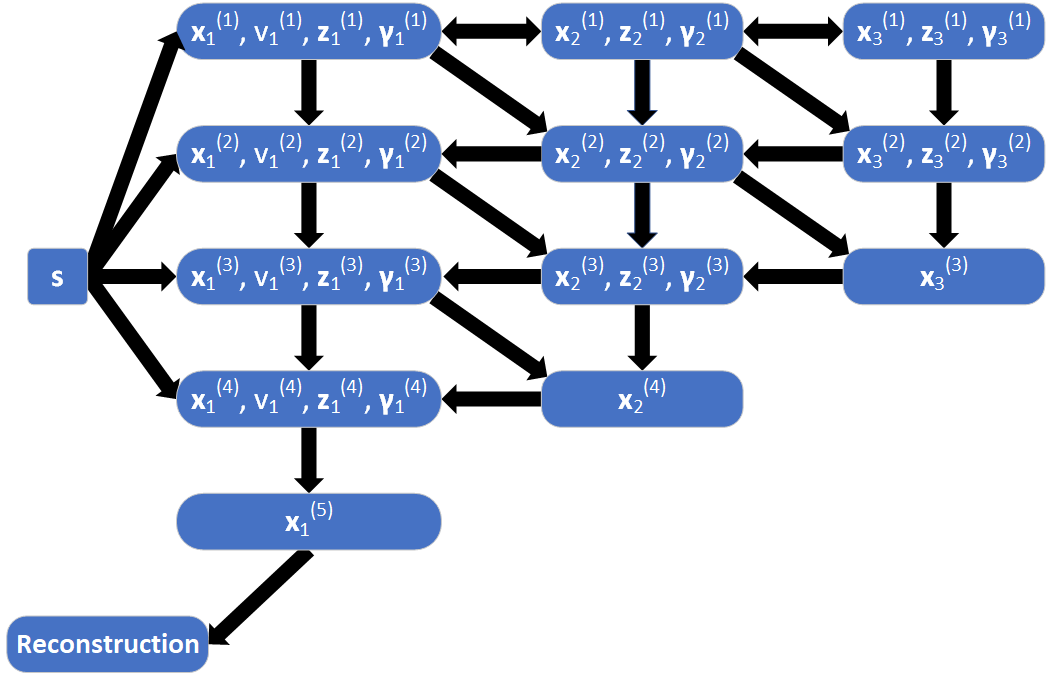
\includegraphics[width=\textwidth]{figures/multi-layer_ADMM-node-dependencies-JPEG.png}
	\caption{This diagram shows interactions between layers across iterations for the ADMM pursuit algorithm applied to JPEG artifact removal. The double-sided arrows at the top of the diagram go both directions because $\vx_{\ell + 1}$ influences $\vz_{\ell}$ during initialization.}
	\label{figure:ADMM Multi-Layer JPEG Diagram}
\end{figure}

\section{Backpropagation Approximation} \label{section:Partial Backprop}
If an iterative sparse coding algorithm converges, after a sufficient number of iterations, the coefficient updates become very small with each iteration, and so the coefficients change very little. Backpropagation can be computationally and memory intensive, and so intuition would suggest backpropagating through steps that are barely even changing the coefficients may not be an optimal use of computational resources. For single-layer dictionary learning, it is very common for practitioners and researchers to iteratively decrease the objective function in respect to the dictionary using gradient methods, treating the coefficients as fixed (rather than a function of the dictionary). Inspired by those methods, I similarly compute approximate gradients without backpropagating through the entire sparse coding algorithm, instead only backpropagating to the last instance of that dictionary's use:\footnote{The last use of $\mD_{\ell + 1}$ occurs in a $\vz_{\ell}$ update, and $\mD_1\vx_1^{(T)}$ approximately reconstructions the original signal.}
\begin{equation}
\nabla_{\mD_1} \loss \approx \nabla_{\mD_1}^{\left(\vx_1^{(T)} \rightarrow \mD_1\vx_1^{(T)}\right)} \loss
\end{equation}
\begin{equation} \label{equation:Partial Backprop}
\nabla_{\mD_{\ell}} \loss \approx \nabla_{\mD_{\ell}}^{\left(\vx_{\ell}^{(T - \ell + 1)} \rightarrow \mD_{\ell}\vx_{\ell}^{(T - \ell + 1)}\right)} \loss
\end{equation}
This approximation\footnote{It may help to recall from Equations \ref{equation:x-update JPEG} and \ref{equation:z-update JPEG} that $\vx_{\ell + 1}^{(t)}$ has no influence on $\vx_{\ell}^{(t)}$; instead, it is used to update $\vz_{\ell}^{(t)}$ which subsequently is used in the $\vx_{\ell}^{(t + 1)}$ update equation. For this reason, Equation \ref{equation:Partial Backprop} depends on $\vx_{\ell}^{(T - \ell + 1}$, not $\vx_{\ell}^{(T)}$. These types of interactions between variables across layers and iterations are shown in Figure \ref{figure:ADMM Multi-Layer JPEG Diagram}.} of the gradient for dictionary learning is used in the experiment detailed in the subsequent section.




\section{Experiment}
In this section, I apply this novel multi-layer dictionary approach to other multi-layer dictionary algorithms on the task of removing artifacts from JPEG compression.
\subsection{Experiment Setup}
The BSDS500 dataset consists of $200$ training images, $100$ validation images, and $200$ test images, and was originally designed to test segmentation algorithms. For this experiment, I compress the images using a quality factor of $25$. For training, the algorithms are given both the compressed and raw images. The images vary in size, so I split the images into smaller $32 \times 32$ patches. For validation and testing, the algorithms are assessed on how well they reconstruct original image patches from the compressed image patches.
\subsection{Network Architecture}
To compare the FISTA and ADMM for multi-layer dictionary learning, both algorithms are set up with the same basic $2$-layer architecture, the details of which are shown in Table \ref{table:JPEG Artifact Removal Architecture}. For both, coefficients of the last layer are constrained to be non-negative.\footnote{For ADMM, this is enforced on the $\vz$ coefficients by adding an indicator function to the objective $\indicator_{\vz_L \geq \vzero}(\vz_L)$.}  The reason I use $\mathbb{L} = 64$ for FISTA is because $\mathbb{L} = 16$ diverged during sparse coding. For dictionary learning, I use stochastic gradient descent for both, using a step-size of $0.01$. Backpropagation is used to learn not just elements of the dictionary, but also the weighting of the penalty terms $\mu_{\ell}$ and $\lambda_{\ell}$. The loss minimized is the mean-squared error of the reconstruction in respect to the raw (pre-compression) images. To reduce computation time and memory usage, backprogagation for the dictionary updates is only computed over the last few computations as described in Section \ref{section:Partial Backprop}.
\begin{table}[] 
\caption{Architecture and Hyper-Parameters for Experiment}
\begin{center}
\begin{tabular}{@{}lllllll@{}}
\toprule
\multicolumn{1}{c}{Algorithm} & \multicolumn{1}{c}{Hyper-Parameter} & \multicolumn{1}{c}{Number of Iterations} & \multicolumn{2}{c}{Number of Filters}                     & \multicolumn{2}{c}{Filter Size}                           \\ %\midrule
      &      &            & \multicolumn{1}{c}{Layer 1} & \multicolumn{1}{c}{Layer 2} & \multicolumn{1}{c}{Layer 1} & \multicolumn{1}{c}{Layer 2} \\ \midrule
ADMM                          & $\rho = 1$, $\reflectbox{R} = 4$                     & 16                        & 32                          & 64                          & $5 \times 5$                & $7 \times 7$                \\
FISTA                         & $\mathbb{L} = 64$                      & 48                            & 32                          & 64                          & $5 \times 5$                & $7 \times 7$                \\ \bottomrule
\label{table:JPEG Artifact Removal Architecture}
\end{tabular}
\end{center}
\end{table}
\subsection{Results}
The decrease in reconstruction error across a validation set for ADMM is shown in Figure \ref{figure:Train Error Curve ADMM}. ADMM is able to reduce the error, improving the dictionary across many updates. A similar curve is shown for FISTA in Figure \ref{figure:Train Error Curve FISTA} trained on the same data for the same number of dictionary updates. The dictionary updates for FISTA fail to reduce the error. FISTA's failure to successfully learn a better dictionary likely stems from its slower convergence in the sparse coding task. Figures \ref{figure:Sparse Coding Error} shows the sparse coding error across multiple iterations (using ADMM's $\vz$ coefficients). ADMM's faster convergence allows it to improve the dictionary without backpropagating through the entire network. Even with three times the number of sparse coding iterations, FISTA is still unable to converge fast enough. To succeed, FISTA would either need to backpropagate further through the network, or add more sparse coding iterations, both of which would further increase needed computational resources.
\begin{figure}
%\centering
\begin{subfigure}{.5\textwidth}
        \centering
	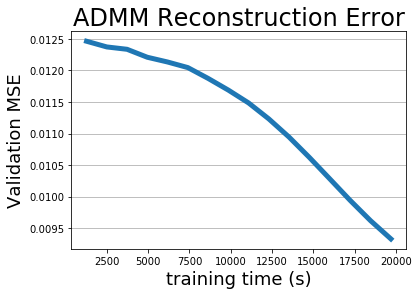
\includegraphics[width=.8\textwidth]{figures/ADMM_Recon_Err.png}
	\caption{ADMM}
	\label{figure:Train Error Curve ADMM}
\end{subfigure}
\begin{subfigure}{.5\textwidth}
        \centering
	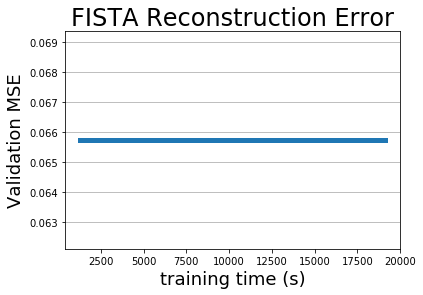
\includegraphics[width=.8\textwidth]{figures/FISTA_Recon_Err.png}
	\caption{FISTA}
	\label{figure:Train Error Curve FISTA}
\end{subfigure}
     \caption{This is the reconstruction error for the multi-layer dictionary model measured on the validation set shown as a function of training time. Subfigure \ref{figure:Train Error Curve ADMM} shows the error for the ADMM algorithm and Subfigure \ref{figure:Train Error Curve FISTA} shows the error for the FISTA algorithm.}
     \label{figure:Train Error Curve}
\end{figure}
\begin{figure}
    \centering
    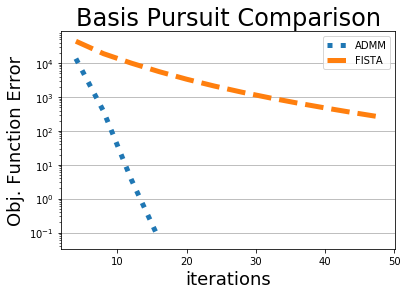
\includegraphics[width=.75\textwidth]{figures/Sparse_Coding_Comparison.png}
    \caption{This plots the objective function from equation \ref{equation:JPEG Sparse Coding Objective} in respect to iterations, using $\vz_{\ell}$ for the coefficients of the ADMM approach.}
    \label{figure:Sparse Coding Error}
\end{figure}
\section{Conclusion}
This chapter showed how to adapt the multi-layer dictionary approach from chapter $3$ to the JPEG artifact removal problem. This involved combining the multi-layer model with the convex indicator function from \cite{sorel2016efficient} to impose the quantization constraints, subtracting out the low-frequency components, and approximating the gradients.  With my novel approach, ADMM handled the gradient approximations better than FISTA did, and demonstrated faster convergence for sparse coding.
